\documentclass{beamer}
\usetheme{Warsaw}

\usepackage[utf8]{inputenc}
\usepackage{fancybox}
\usepackage{multimedia} 
\usepackage{subfig}
\usepackage{amsmath}
\usepackage{hyperref}
\usepackage{marvosym}

\usepackage[all]{xy}
\begin{document}


\title[Digitale Bildverarbeitung] % (optional, only for long titles)
{Digitale Bildverarbeitung
\\
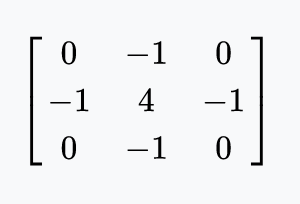
\includegraphics[scale=1.0]{img/cover}
}
\subtitle{}
\author[Dr. Johannes Riesterer] % (optional, for multiple authors)
{Dr.  rer. nat. Johannes Riesterer}

\date[KPT 2004] % (optional)
{}

\subject{Digitale Bildverarbeitung}

\frame{\titlepage}


\begin{frame}
    \frametitle{Integration}
\framesubtitle{}

    \begin{block}{Integral}
Sei $A \subseteq \mathbb{R} \times \mathbb{R}$ eine (meßbare) Teilmenge und  $f: \mathbb{A} \to \mathbb{R}$ eine (meßbare, integrierbare) Funktion.
Dann können wir das Integral definieren durch
\begin{align*}
\int_A f  \; d (x,y) \;  := \int_{A_x} \Biggl( \int_{A_y} f(x,y) \;  dx \Biggr) \; dy 
\end{align*}
mit den Scheibenmengen $A_y := \{x \in \mathbb{R} \;  | \, (x,y) \in A \}$ und $A_x =  \{y \in \mathbb{R} \;  | \, A = \bigcup_y A_y \}$
\end{block}

 \end{frame}


\begin{frame}
    \frametitle{Integration}
\framesubtitle{}

    \begin{block}{Integral}
Induktiv definieren wir dann  für eine Funktion $f: \mathbb{A} \subset \mathbb{R}^n \to \mathbb{R}$
das Integral  durch
\begin{align*}
\int_A f(x)  \; dx\;  := \int_{A_{1}} \cdots \int_{A_{n}} f(x_1, \ldots,   x_n) \;  dx_1  \;  \cdots \; dx_n 
\end{align*}

\end{block}

 \end{frame}


\begin{frame}
    \frametitle{Integration}
\framesubtitle{}

    \begin{block}{Volumen}
Für $A \subseteq \mathbb{R}^n $  definieren wir das Volumen  durch
\begin{align*}
\mu(A) := \int_A 1  \; dx  
\end{align*}
\end{block}
 \end{frame}


\begin{frame}
    \frametitle{Integration}
\framesubtitle{}

    \begin{block}{Beispiel}
$A:= \{ (x,y) \in \mathbb{R}^2 \;  | \;  x^2 + y^2 \leq 1\}$ (Kreisscheibe). $A_x =  \{ y  \in \mathbb{R} \;  | \; -1 \leq y \leq 1\} $
$A_y =  \{ x  \in \mathbb{R} \;  | \;  -\sqrt{1 - y^2} \leq x \leq \sqrt{1 - y^2} \} $
\end{block}
\begin{figure}[htp]
      \centering
    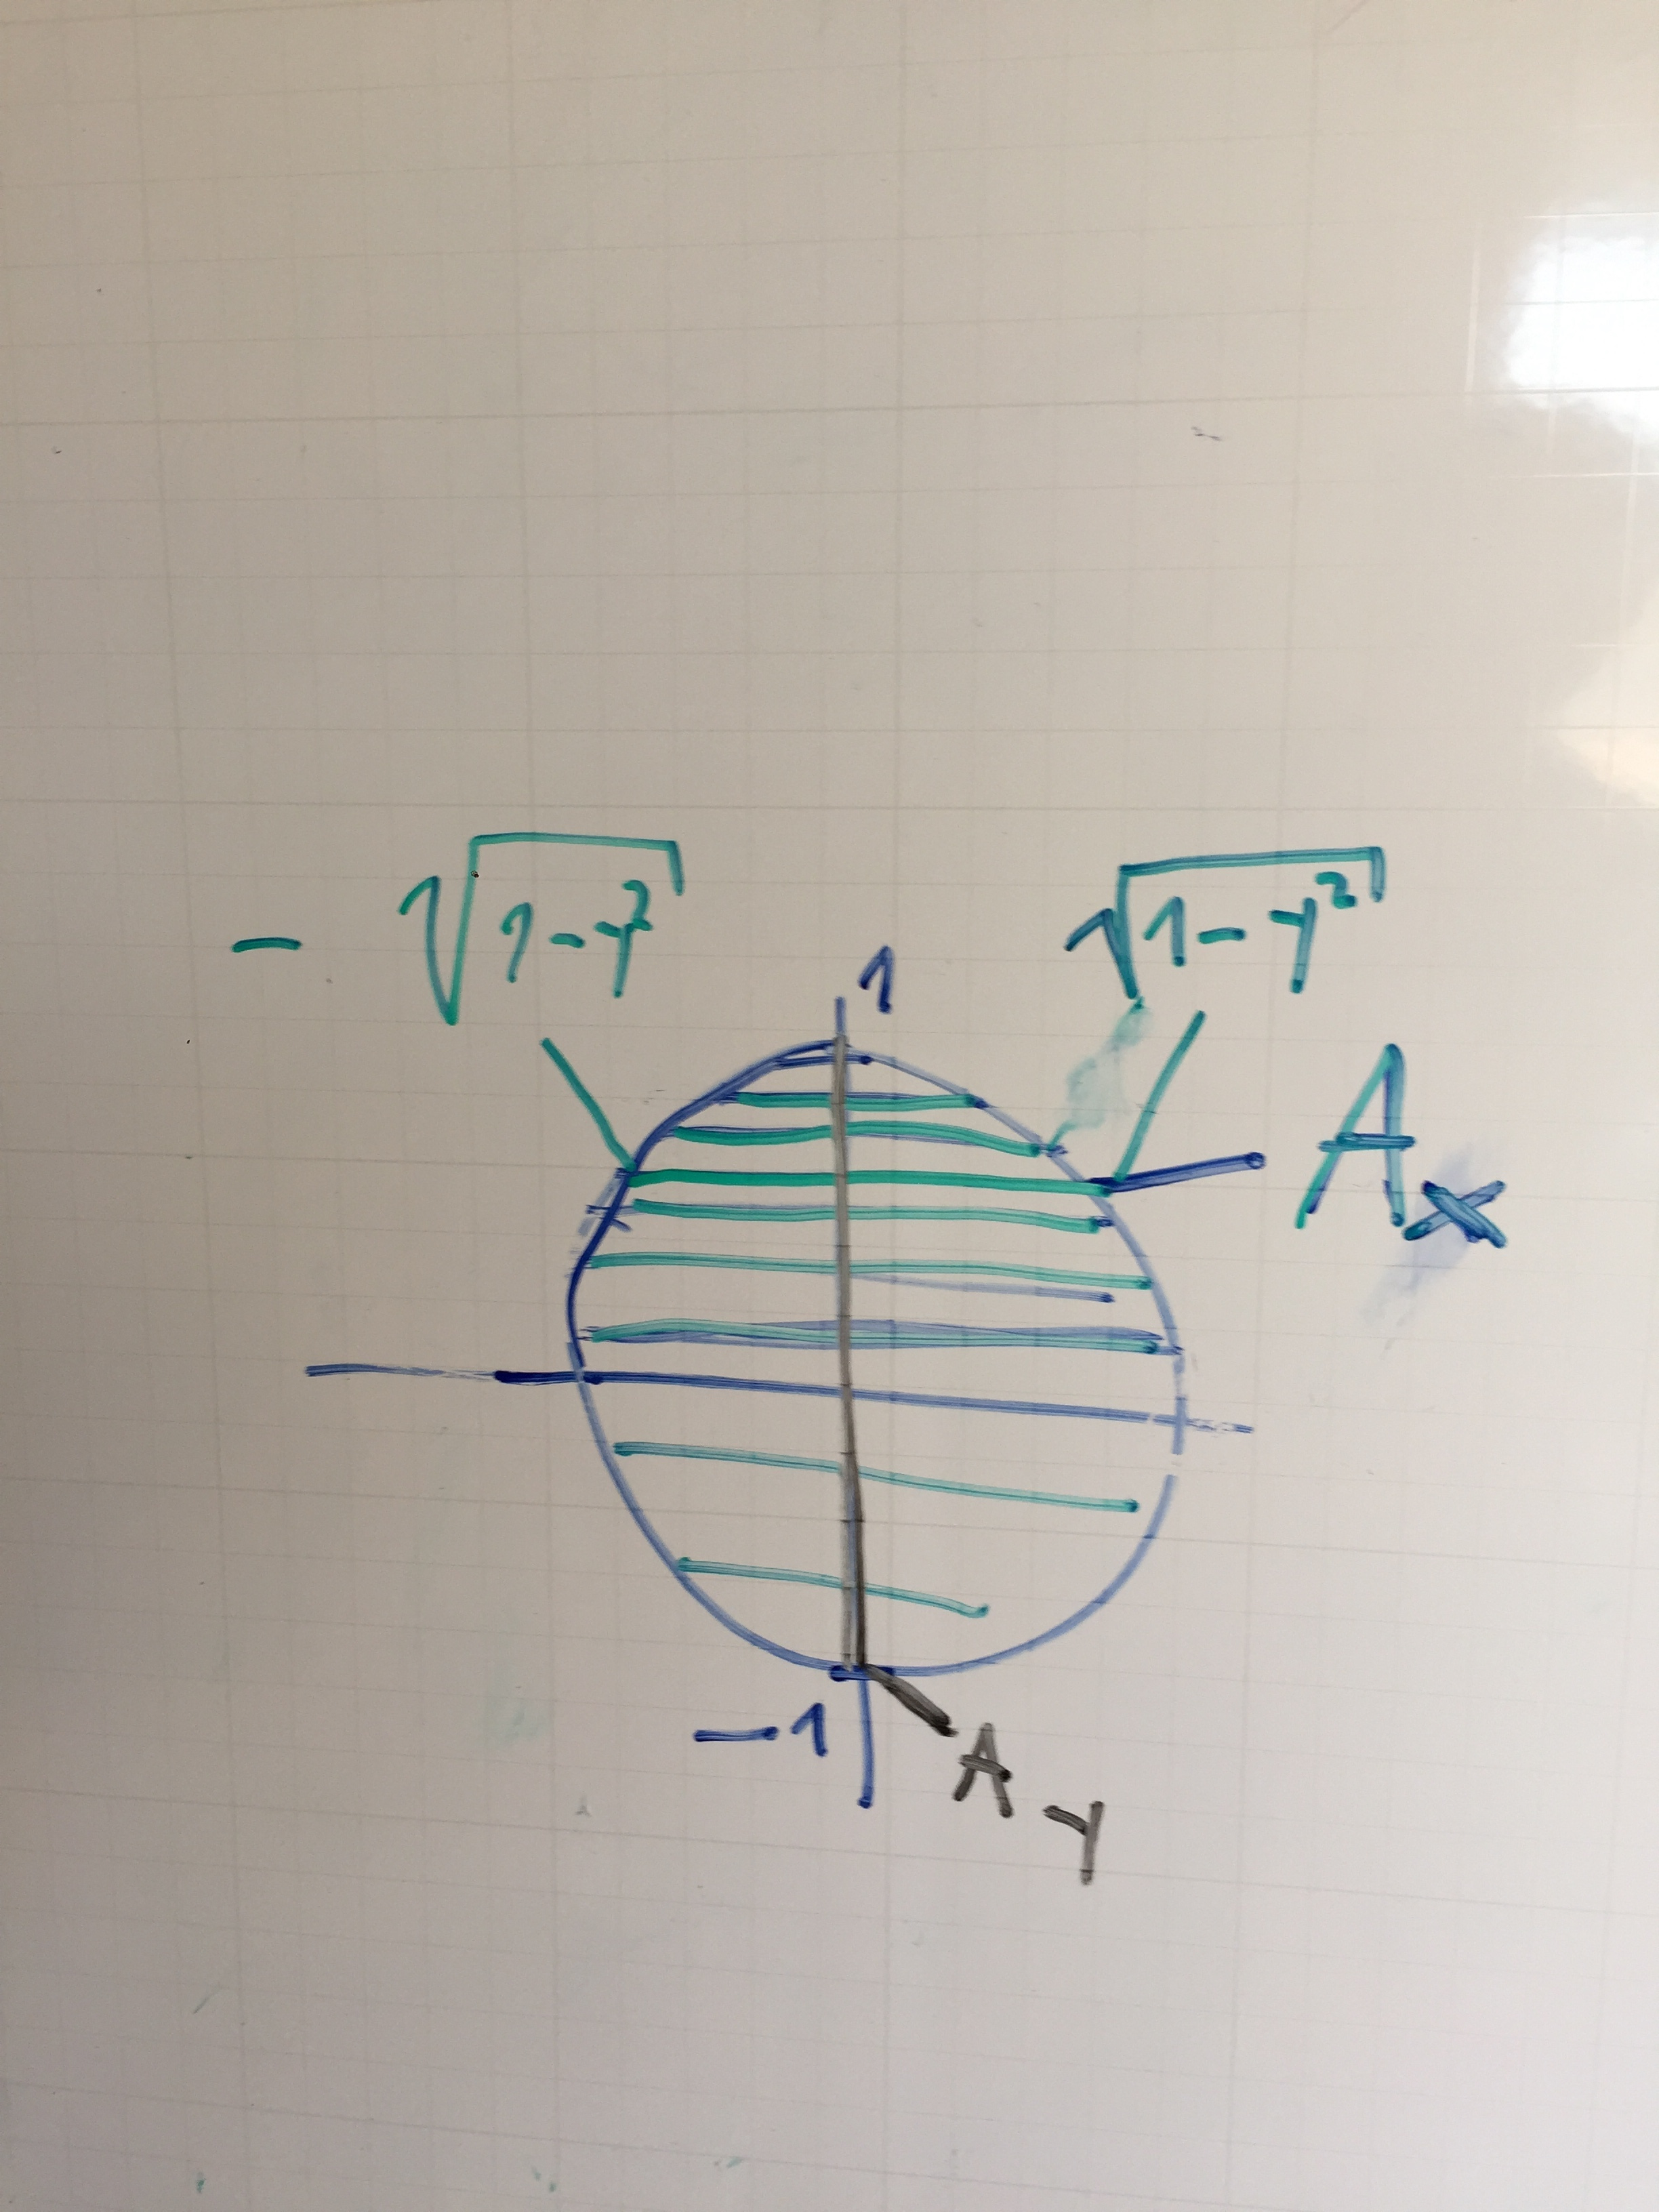
\includegraphics[width=0.35\textwidth]{img/int}
      \caption{Scheibenmengen}
\end{figure}
 \end{frame}

\begin{frame}
    \frametitle{Integration}
\framesubtitle{}

    \begin{block}{Beispiel}
\begin{align*}
\mu(A) = & \int_A 1  \; d(x,y) \;  := \int_{-1}^{1} \Biggl( \int_{-\sqrt{1 - y^2} }^{\sqrt{1 - y^2} } 1 \;  dx \Biggr) \; dy \\ 
& =  2 \int_{-1}^{1}  \sqrt{1 - y^2}   \; dy  \\ 
 & (substitution \;   y = sin(u)) =   2 \int_{-\frac{\pi}{2}}^{\frac{\pi}{2}}   \cos(u)^2   \; du = 2 \cdot \frac{\pi}{2} = \pi
\end{align*}
\end{block}

 \end{frame}


\begin{frame}
    \frametitle{Punktoperationen}
\framesubtitle{}

    \begin{block}{Histogramm}
Für ein diskretes Bild $U : \Omega \to R$ beziehungsweise für ein kontinuierliches Bild $u: \Omega \to R$  definieren wir das Histogramm 
\begin{align*}
& H_U (k): = \#\{  i \in \Omega | U_i = k \} \\
& H_u (E): = \mu (\{  x \in \Omega |  u(x) \in  E \} ), \; E \subset R 
\end{align*}
\end{block}

    \begin{block}{Verteilungsfunktion}
Ebenso definieren wir die Verteilungsfunktion
\begin{align*}
& G_U (s): = \# \{  i \in \Omega |  u_i \leq  s \} \\
& G_u (s): = \mu ( \{  x \in \Omega |  u(x) \leq  s \} )
\end{align*}
\end{block}


    \begin{block}{Bemerkung}
Für $R = [0,1]$ ist
$H_u ([0,1])= \mu (\Omega)$
\end{block}


 \end{frame}



\begin{frame}
    \frametitle{Punktoperationen}
\framesubtitle{}

    \begin{block}{Histogrammausgleich}
Ein Bild mit viel Kontrast hat Grauwerte im gesamten Bereich $R = [0,1]$. Man ist daher daran interessiert, Abbildungen des Bildes zu finden, so  dass das Histogramm des abgebildeten 
Bildes möglichst gleichmässig verteilt ist.  
\end{block}

   \begin{block}{Einfacher Histogrammausgleich}
die Abbildung  
 \begin{align*}
\phi : [0,1] \to [0,1] \\
\phi(s) = \frac{s -inf(u)}{sup(u) - inf(u)}
\end{align*}
spreizt das Histogramm des Bildes auf den gesamten Bereich $[0,1]$ und erhöht daher insgesamt den Kontrast.
\end{block}

 \end{frame}



\begin{frame}
    \frametitle{Punktoperationen}
\framesubtitle{}

    \begin{block}{Histogrammausgleich}
Wir suchen eine  monotone Abbildung $\psi :[0,1] \to [0,1]$ mit
 \begin{align*}
&H_{\psi \circ u} ([a,b]) =  (b-a)\mu(\Omega) \\
\Leftrightarrow & G_{\psi \circ u} (s) = s \mu(\Omega)
\end{align*}
\end{block}

    \begin{block}{Histogrammausgleich}
Nehmen wir an, dass $\psi$ invertierter ist, ergibt sich
 \begin{align*}
 s \mu(\Omega) & =  \mu ( \{  x \in \Omega | \psi( u(x)) \leq  s \} ) \\
 & =  \mu ( \{  x \in \Omega |  u(x) \leq  \psi^{-1} (s )\} ) \\
& = G_{u}(\psi^{-1} (s ))
\end{align*}
und damit $\psi^{-1} (s ) = G_u^{-1} (s \mu(\Omega))$ und also
$\psi(s) = \frac{G_u(s)}{\mu(\Omega)}$.
\end{block}



 \end{frame}




\begin{frame}
    \frametitle{Integration}
\framesubtitle{}

    \begin{block}{Faltung}
\begin{align}
(f * g )(x) := \int_{\mathbb{R}^n}  f(y-x) \cdot g(y) \; dy 
\end{align}

\end{block}
    \begin{block}{Beispiel 1}
\href{https://moodle.dhbw-mannheim.de/pluginfile.php/278535/mod_folder/content/0/Convolution_of_box_signal_with_itself.gif?forcedownload=1}{Link: Box}
\end{block}
 
    \begin{block}{Beispiel 2}
\href{https://moodle.dhbw-mannheim.de/pluginfile.php/278535/mod_folder/content/0/Convolution_Animation_(Gaussian).gif?forcedownload=1}{Link: Gauß}
\end{block}
 
\end{frame}


\begin{frame}
    \frametitle{Diskrete Faltung}
\framesubtitle{}

    \begin{block}{Diskrete Faltung}
Für zwei diskrete  Funktionen $U : [1, \ldots, N]  \to R$ und $H : [1, \ldots, N]  \to R$ mit stückweisen konstanten Interpolation $u(x) := \sum_{l=1}^{N} U_l \phi^0_j(x)$ und 
$h(x) := \sum_{m=1}^{N} H_m \phi^0_m(x)$ ergibt die Faltung 
\begin{align*}
& (h * u)(k) = \int u(y)h(k-y)  \; dy \\
& = \int \ \sum_{l=1}^{N} U_l \phi^0(y-l) \sum_{m=1}^{N} H_m \phi^0(k-y-m) \\
& = \sum_{l=1}^{N}   \sum_{m=1}^{N} U_l  H_m  \int  \phi^0(y-l) \phi^0(k-y-m) \; dy 
\end{align*}

\end{block}
 \end{frame}

\begin{frame}
    \frametitle{Diskrete Faltung}
\framesubtitle{}

    \begin{block}{Diskrete Faltung}
Da für das Integral 
\begin{align*}
  \int  \phi^0(y-l) \phi^0(k-y-m)  \; dy  = \begin{cases}
1 \text{ falls } m = k -l\\
0 \text{ sonst }
\end{cases}
\end{align*}
gilt, folgt die Darstellung
\begin{align*}
 (u  * h)(k) = \sum_l U_l H_{k-l}
\end{align*}

\end{block}

 \end{frame}




\end{document}
